\documentclass[slidetop, mathserif]{beamer}

% \mode<presentation>
% {
% 	\usetheme{Warsaw}
% 	\setbeamercovered{transparent}
% }

% \usepackage{caption}
\usepackage{subcaption}
\captionsetup{compatibility=false}


\mode<presentation>{
	\usetheme{Berlin}
	\setbeamercovered{transparent}
	\usefonttheme{professionalfonts}
}

\usepackage{amsmath, amsfonts, amssymb}
\usepackage{mathrsfs,dsfont}

\newcommand{\norm}[1]{\left\|#1\right\|}
\newcommand{\suchthat}{-\hspace{-10pt}\ni\hspace{-10pt}-}


\AtBeginSection[]
{
   \begin{frame}
       \tableofcontents[currentsection]
   \end{frame}
}

%% want to use verbatim: \begin{frame}[fragile]

\title[Metrics for Tracking]{Metrics for Trackings: Evaluations and Comparisons}
\author[chy1010]{Chien, Hung-Yu (chy1010) \\ {\tt andy1010@gmail.com}}
\date{\today}

\begin{document}

\frame{\titlepage}

\section[Outline]{}
\begin{frame}
    \frametitle{Outlines}
    \tableofcontents
\end{frame}

\section{Preliminaries}

\begin{frame}
	\frametitle{MOT (Multiple Object Tracking)}
	
	Given a video, the task of MOT consists of the following parts:
	\begin{itemize}
		\item locating multiple objects,
		\item maintaining their identities, and
		\item yielding their individual trajectories.
	\end{itemize}
	
	In more details, \emph{each object is assigned a unique id in a frame.}
	And objects with the same id in consecutive frames form a trajectory.
	
	\begin{figure}
		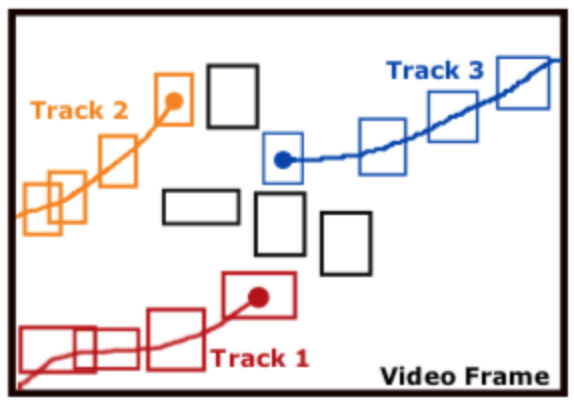
\includegraphics[height=70pt]{pics/fig1.png}
		\caption{objects with the same id from different frames}
	\end{figure}
	
\end{frame}

\begin{frame}
	\frametitle{To Evaluate the MOT Results}
	
	Whatever how we perform tracking the same objects in a sequence of frames.
	New nominal ids are assigned to detected objects in every frames.
	
	Hence to compare the results with the ground-truth data, we need to match the new ids
	with the original ids.
	
	The matchings are done in different levels such as:
	\begin{itemize}
		\item {\bf frame levels / detection levels}:
		      match ground-truth objects (denoted by gtDets)
		      with predictions (denoted by prDets) frame by frame.
		\item {\bf sequence levels / trajectory levels}:
		      match each ground-truth id to an hypothesis id along a sequence of frames.
	\end{itemize}
	
\end{frame}

\begin{frame}
	\frametitle{Matching in Frame-Levels}
	
	Here a {\bf matching} is a \emph{1-1 relation} between ground-truths
	and predictions in the same frame.
	It can be done by according to the {\bf similarities} of every `gt-pred' pair.
	For example, $\max\{1-\text{\tt dist}, 0\}$ and {\tt IoU} are metrics for
	measuring similarity, which is in $[0,1]$.
	
	\vspace{4pt}
	
	Denote $\mathcal S(g_i, p_j)$ be the similarity score of $i$-th ground-truth object
	and $j$-th prediction. Let $\alpha\in(0,1)$.
	Then a matching $\Pi$ under the similarity threshold $\alpha$ is a 1-1 relation
	satisfying
	\[
		(g,p) \in \Pi \Rightarrow \mathcal S(g, p) \geq \alpha. ~ \text{($g$, $p$ must belong the same frame.)}
	\]
	
	% \vspace{2pt}
	
	\emph{1-1 relation: if $(g_i, p_j)$, $(g_k, p_\ell)\in \Pi$,
		then $i=k$ $\Leftrightarrow$ $j=\ell$.}
	
\end{frame}

\begin{frame}
	\frametitle{Trivial Notions}
	
	\begin{itemize}
		\item Denote $F:=\{f_0, f_1, \ldots, f_{N-1}\}$ as the set of frames.
		\item If $\Pi$ is a matching, it can be a matching in a frame $f$ and specified by $\Pi^{(f)}$;
		      or be a matching during all frames.
		\item When $\Pi$ denotes a global matching, it is the union of all its sections:
		      $\Pi = \cup_{f\in F}\Pi^{(f)}$.
		\item Furthermore, once a collection $E$ is well-defined in each frame,
		      we denote $E^{(f)}$ as the $f$-section, i.e. elements in frame $f$.
		      
	\end{itemize}
	
	For a ground-truths $g$ or a prediction $p$, denote
	\begin{itemize}
		\item $f_g$ / $f_p$ as the frame it appears;
		\item $\text{gtId}(g)$ / $\text{prId}(p)$ as its id;
		\item $\text{gtTr}(g)$ / $\text{prTr}(p)$ as its trajectory (objects with the same id).
	\end{itemize}
\end{frame}

\begin{frame}
	\frametitle{TP, FP and FN}
	
	For a given matching $\Pi$ during all frames, we can define:
	\begin{itemize} \itemsep = 2pt
		\item TP, $\text{TP}_\Pi$ (true positive cases): Matched pairs in $\Pi$.
		\item FP, $\text{FP}_\Pi$ (false positive cases): Non-matched predictions.
		\item FN, $\text{FN}_\Pi$ (false negative cases): Non-matched ground-truths.
	\end{itemize}
	
	\begin{figure}
		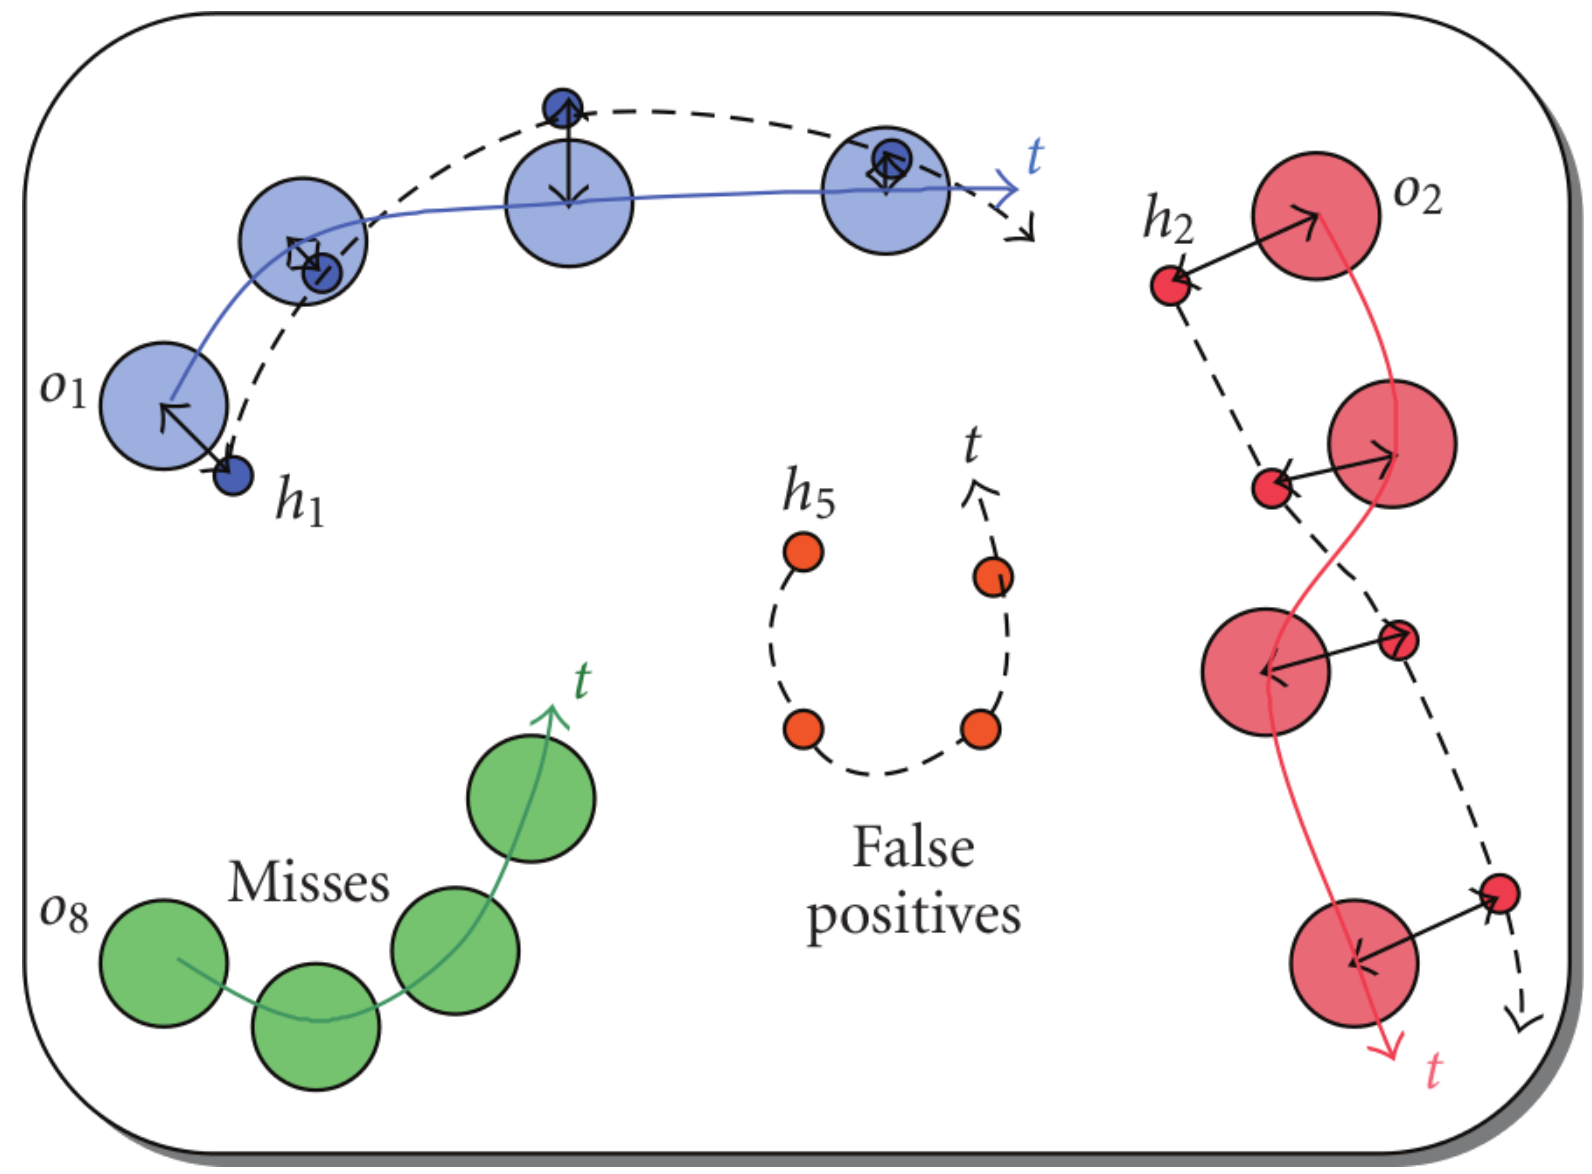
\includegraphics[width=120pt]{pics/fig2.png}
		\caption{TP's, FP's, FN's in consecutive frames.}
	\end{figure}
	
\end{frame}

\begin{frame}
	\frametitle{IDSW in Consecutive Frames}
	
	An {\bf IDSW (id switch)} event means there exist TP pairs, say $(g_i, p_j)\in\Pi^{(f)}$,
	$(g_k, p_\ell)\in\Pi^{(f+1)}$, in two consecutive frames
	$f$ and $f+1$ that satisfy
	\[
		\text{gtId}(g_i) = \text{gtId}(g_k),\ 
		\text{prId}(p_j) \neq \text{gtId}(p_\ell).
	\]
	Actually, this is an \emph{id mismatch} occuring in frame $f+1$.
	If two objects exchange their ids in new frame, then this is regarded as $2$
	IDSW events.
	\begin{figure}
		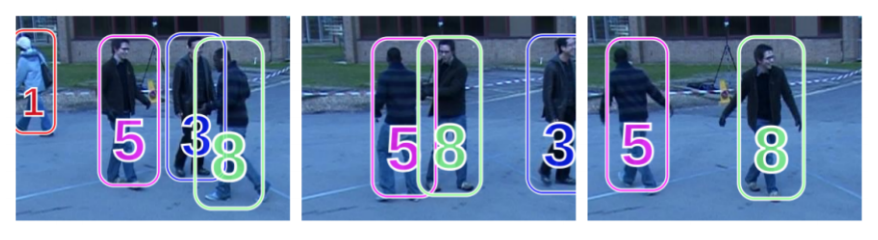
\includegraphics[width=180pt]{pics/fig3.png}
		\caption{The ids 3 \& 8 exchanges. 2 IDSW events.}
	\end{figure}
	    
	    
\end{frame}

\begin{frame}
	\frametitle{Matching in Sequence-Levels}
	    
	Matchings in sequence-levels are done by associating one ground-truth trajectory
	% ({\tt gtTraj})
	to exactly one predictive trajectory
	% ({\tt prTraj})
	along a sequence of frames.
	Denote such matchings by swash fonts $\mathfrak P$.
	    
	\quad
	
	% The similarity of a {\tt grTraj} and a {\tt prTraj} is often divided into
	% different levels: `mostly tracked' and `mostly lost'.
	Note that \emph{the similarities of two trajectories still depend on the
	framewise matching under some threshold.}
	When most objects are matched, then we call it `mostly tracked';
	Otherwise, we call it `mostly lost'.
	% Here it is usually defined in a Jaccard index (IoU) way:
	% \[
	%     \mathcal S_{\rm tr}(\text{\scriptsize gtTraj}, \text{\scriptsize prTraj}, \Pi_\alpha) =
	%         |\text{TP}| / (|\text{TP}|+|\text{FN}|+|\text{FP}|).
	% \]
	\begin{figure}
		\begin{subfigure}{.5\textwidth}
			\centering
			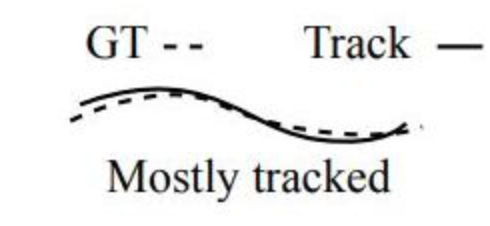
\includegraphics[width=80pt]{pics/fig4.png}
		\end{subfigure}%
		\begin{subfigure}{.5\textwidth}
			\centering
			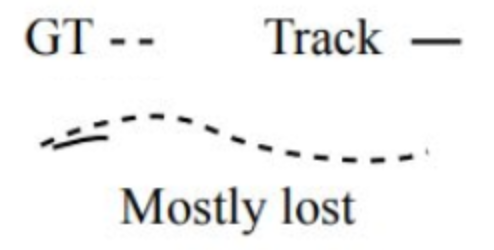
\includegraphics[width=70pt]{pics/fig5.png}
		\end{subfigure}
		\caption{Mostly tracked \& mostly lost.}
	\end{figure}
	
\end{frame}


\begin{frame}
	\frametitle{Similarity of Trajectories}
	
	To measure the similarity of trajectories, we need to evaluate the 
	overlapping and non-overlapping parts of them.
	
	\vspace{4pt}
	
	Let $\mathfrak g$, $\mathfrak p$ be a pair of trajectories
	and $\alpha$ be a (detection-) similarity threhold.
	We can define $\mathcal{TP}$'s, $\mathcal{FP}$'s, and $\mathcal{FN}$'s for overlapping of trajectories.
	\begin{itemize}
		\item $\mathcal{TP}$, $\mathcal{TP}_{\mathfrak g, \mathfrak p}$:
		      the overlapping part of $\mathfrak g$ and $\mathfrak p$.
		      \[
		      	\mathcal{TP} := \{(g,p)\ |\ 
		      	g\in\mathfrak g,~
		      	p\in\mathfrak p,~
		      	f_g=f_p,~ \mathcal S(g,p)\geq \alpha\}
		      \]
		\item $\mathcal{FP}$, $\mathcal{FP}_{\mathfrak g, \mathfrak p}$:
		      the non-matched predictions.
		      \begin{align*}
		      	\mathcal{FP} := & \{ p\in\mathfrak p\ |\ 
		      	\nexists\ g\in\mathfrak g ~\suchthat~ \mathcal S(g,p)\geq\alpha.\}
		      \end{align*}
	\end{itemize}
	
\end{frame}

\begin{frame}
	\frametitle{Similarity of Trajectories}
	
	\begin{itemize}
		\item $\mathcal{FN}$, $\mathcal{FN}_{\mathfrak g, \mathfrak p}$: the non-matched ground-truth objects.
		      \begin{align*}
		      	\mathcal{FN} := & \{ g\in\mathfrak g\ |\ 
		      	\nexists\ p\in\mathfrak p ~\suchthat~ \mathcal S(g,p)\geq\alpha.\}
		      \end{align*}
	\end{itemize}
	
	Hence the similarity is defined in a Jaccard index way:
	\[
		\mathcal S_{\rm tr}(\mathfrak g, \mathfrak p) :=
		\dfrac{|\mathcal{TP}_{\mathfrak g,\mathfrak p}|}{
			|\mathcal{TP}_{\mathfrak g,\mathfrak p}|+|\mathcal{FP}_{\mathfrak g,\mathfrak p}|+|\mathcal{FN}_{\mathfrak g,\mathfrak p}|
		}.
	\]
	Once the similarities are calculated,
	the matching of trajectories can be done by considering the similarities.
\end{frame}


\begin{frame}
	\frametitle{Measures for Id Tracking: IDTP, IDFP, IDFN}
	
	Suppose a matching between ground-truths and predictions are done and denoted by $\mathfrak P$,
	we can define the performance measures as follows.
	
	\vspace{4pt}
	
	Again, denote $\alpha$ as the (detection-) similarity threshold.
	\begin{itemize}
		\item IDTP:
		      the overlapping part of all $(\mathfrak g, \mathfrak p) \in \mathfrak P$.
	\end{itemize}
	
	\vspace{-15pt}
	\[
		\text{IDTP} := \left\{ (g,p)\ |\ 
		g\in\mathfrak g, ~ p\in\mathfrak p, ~
		f_g=f_p, ~ 
		\mathcal S(g,p) \geq \alpha\ 
		\forall\ (\mathfrak g, \mathfrak p)\in\mathfrak P
		\right\}
	\]
	\vspace{-10pt}
	\begin{itemize}
		\item IDFP:
		      non-matched predictions in matched pairs
		      and all predictions in non-matched predictive trajectories.
	\end{itemize}
	    
\end{frame}

\begin{frame}
	\frametitle{Measures for Id Tracking: IDTP, IDFP, IDFN}
	    
	\begin{align*}
		\text{IDFP} := & \left\{ p\in\text{prDets}\ \left|\                                                
		\mathcal S(g,p)<\alpha, \ 
		\forall\ g\in\mathfrak g^{(f_p)},
		(\mathfrak g,\mathfrak p)\in\mathfrak P.
		\right.
		\right\} \\
		               & \bigcup \left\{p \in \text{prDets}\ |\ \text{prTraj$(p)$ is not matched.}\right\} 
	\end{align*}
	
	\vspace{-10pt}
	\begin{itemize}
		\item IDFN:
		      non-matched ground-truths in matched pairs and
		      all ground-truths in non-matched ground-truth trajectories.
	\end{itemize}
	\begin{align*}
		\text{IDFN} := & \left\{ g\in\text{gtDets}\ \left|\                                                
		\mathcal S(g,p)<\alpha, \ 
		\forall\ p\in\mathfrak p^{(f_g)},
		(\mathfrak g,\mathfrak p)\in\mathfrak P
		\right.
		\right\} \\
		               & \bigcup \left\{g \in \text{gtDets}\ |\ \text{gtTraj$(g)$ is not matched}\right\}. 
	\end{align*}
\end{frame}

\begin{frame}
	\frametitle{Problems in Matching Trajectories}
	
	\begin{itemize}
		\item {\bf fragmentations}:
		      A ground-turth trajectory may be matched
		      to several predictive trajectories.
		\item {\bf merge}:
		      A preditive trajectory may be matched to several ground-truth trajectories.
	\end{itemize}
	In both cases, the tracking results are good enough peicewisely,
	but id mismatches occur at several frames.
	Matching in sequence levels only allows 1-1 relation
	between the two kinds of trajectories.
	
	\vspace{4pt}
	
	Hence in the following, we have some quantities to measure
	the overlapping of trajectories in the detection levels.
	This aims to give some partial credits to non-matched good trackers.
	
\end{frame}

\begin{frame}
	\frametitle{Measures for Associations of Objects}
	
	By the concepts of matching in sequence-levels,
	we can further evaluate {\bf tracking associations of an single object}
	along its ground-truth trajectory and predictive trajectory.
	{\color{red} Here the TP's, FP's and FN's are determined in framewise detection levels.}
	
	\vspace{4pt}
	
	Given a frame-level matching $\Pi$.
	Let $c = (g,p)$ be a TP pair in some frame $t$. We can define the true positive
	associations by:
	\begin{align*}
		\text{TPA}(c) :=                       
		\left\{(g_i, p_j)\in\text{TP}\ \left|\ 
		\begin{array}{c}                       
		\text{grId}(g_i)=\text{grId}(g),       \\
		\text{prId}(p_j) = \text{prId}(p)      
		\end{array}\right.                     
		\right\}.                              
	\end{align*}
	Note that $|\text{TPA}(c)|$ is just the number of frames that $\text{gtTraj}(g)$
	and $\text{prTraj}(p)$ overlap.
	
\end{frame}

\begin{frame}
	\frametitle{Measures for Associations}
	
	Similarly, for the TP pair $c = (g, p)$, we also define the false positive associations
	and false negative associations as follows.
	\begin{align*}
		\text{FPA}(c) := &             
		\left\{(g_i, p_j)\in\text{TP}\ \left|\ 
		\begin{array}{c}
		\text{grId}(g_i) \neq \text{grId}(g), \\
		\text{prId}(p_j) = \text{prId}(p)
		\end{array}\right.
		\right\} \\
		                 & ~ \bigcup ~ 
		\Big\{p_j\in\text{FP}\ |\ 
		\text{prId}(p_j) = \text{prId}(p)
		\Big\}; \\
		\text{FNA}(c) := &             
		\left\{(g_i, p_j)\in\text{TP}\ \left|\ 
		\begin{array}{c}
		\text{grId}(g_i) = \text{grId}(g), \\
		\text{prId}(p_j) \neq \text{prId}(p)
		\end{array}\right.
		\right\} \\
		                 & ~ \bigcup ~ 
		\Big\{g_i\in\text{FN}\ |\ 
		\text{gtId}(g_i) = \text{gtId}(g)
		\Big\}.
	\end{align*}
	Note that $\text{FPA}(c)$ and $\text{FNA}(c)$ relate to the non-matched or id-mismatched
	objects in $\text{prTraj}(p)$ and $\text{grTraj}(g)$.
	
\end{frame}

% \begin{frame}
%     In the next section,
%     we'll introduce metrics for measuring tracking results
%     via the defined quantities.

% \end{frame}

\section{Metrics for Measuring Tracking Results}

\begin{frame}
	\frametitle{Metrics for Measuring Tracking Results}
	
	Performance of object trackings is based on the result of detections.
	
	\quad 
	
	To measure the results, the metrics often consists of the following aspects
	\begin{itemize}
		\item detection;%: measure accuracies of predictions
		\item localization;%: measure accuracies of positions of correct predictions
		\item association.%: measure accuracies of the correct associations of objects
	\end{itemize}
	    
\end{frame}

\subsection{CLEAR-MOT: MOTA and MOTP}

\begin{frame}
	\frametitle{CLEAR-MOT: MOTA and MOTP}
	
	% {\scriptsize\tt K. Bernardin \& R. Stiefelhagen, Evaluating Multiple Object Tracking Performance:%
	% The CLEAR MOT Metrics.}
	
	Given a similarity threshold $\alpha$.
	
	\quad
	
	{\bf MOTA (multiple object tracking accuracy)} is calculated through optimizing the value
	\[
		\text{MOTA}_\alpha :=
		\max_{\Pi_\alpha}
		\left\{1 - \dfrac{|\text{FN}_{\Pi_\alpha}| + |\text{FP}_{\Pi_\alpha}| + |\text{IDSW}_{\Pi_\alpha}|}{|\text{gtDet}|}\right\}
	\]
	among all matchings $\Pi_\alpha$ with $\mathcal S(c)\geq \alpha$ for all matched $c\in\Pi_\alpha$.
	
	\quad
	
	Note that here the matching is done in frame-levels.
	{\bf\color{blue} FN, FP terms measure the accuracy of detections.}
	{\bf\color{olive} The IDSW term measures the accuracy of id-associations.}
	
\end{frame}

\begin{frame}
	\frametitle{CLEAR-MOT: MOTA and MOTP}
	
	As MOTA is achieved by some matching $\Pi_\alpha$, {\bf MOTP (multiple object tracking precision)}
	is calculated as follows:
	\[
		\text{MOTP}_\alpha =
		\dfrac{\sum_{(g,p)\in\text{TP}_{\Pi_\alpha}}\mathcal S(g,p)}{|\text{TP}_{\Pi_\alpha}|}.
	\]
	
	\quad 
	
	Note that {\bf\color{red} MOTP measures the accuracy of localizations of predictions}.
	
	By direct observations, if the MOTA value is low,
	then somehow it cannot be distinguished that
	the detections are not good or the tracking results are not good.
	
	
\end{frame}

\subsection{Performance Measures for MTMCT: the ID Metrics}

\begin{frame}
	\frametitle{The ID Metrics}
	
	As a measure for the {\bf MTMCT (multi-target, multi-camera tracking)} tasks,
	the id metrics focus on matching of trajectories.
	
	\quad 
	
	Under a similarity threshold $\alpha$, the scoring functions are calculated through optimizing
	the quantity $|\text{IDTP}|$ by matching in sequence-levels as follows:
	\begin{align*}
		\text{ID-Precision} := & ~ \max_{\mathfrak P} \dfrac{|\text{IDTP}|}{|\text{IDTP}| + |\text{IDFP}|}, \\
		\text{ID-Recall} :=    & ~ \max_{\mathfrak P}\dfrac{|\text{IDTP}|}{|\text{IDTP}| + |\text{IDFN}|},  \\
		\text{IDF1} :=         &                                                                            
		~ \max_{\mathfrak P}\dfrac{|\text{IDTP}|}{|\text{IDTP}| + 0.5|\text{IDFP}| + 0.5|\text{IDFN}|}.
	\end{align*}
	
\end{frame}

\begin{frame}
	\frametitle{The ID Metrics}
	
	By direct observations, these id metrics show how good the whole tracking trajectories are.
	But once if several fragmentations occur in different frames,
	then we cannot not distinguish this case with the mostly lost cases.
	
	\begin{figure}
		\begin{subfigure}{.5\textwidth}
			\centering
			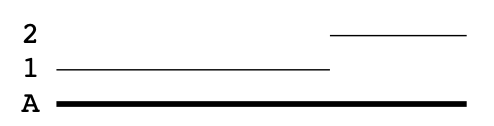
\includegraphics[width=120pt]{pics/fig6.png}
		\end{subfigure}%
		\begin{subfigure}{.5\textwidth}
			\centering
			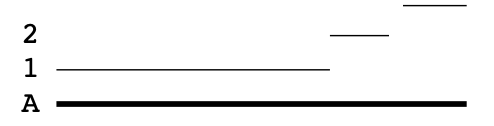
\includegraphics[width=120pt]{pics/fig7.png}
		\end{subfigure}
		\caption{The id metrics only measure tracking results of matched peices.
		The ground-truth id is shown by the bold line.}
	\end{figure}
	
\end{frame}

\subsection{A Higher Order Metric for Tracking Accuracy: the HOTA metric}

\begin{frame}
    \frametitle{The HOTA metrics}

    The HOTA score for a particular similarity threshold $\alpha$ is defined by
    optimizing among matchings in detection levels:
    \[
        \text{HOTA}_\alpha := 
        \max_{\Pi_\alpha} \sqrt{\dfrac{\sum_{c\in\text{TP}} \mathcal A(c) }{|\text{TP}|+|\text{FN}|+|\text{FP}|}},
    \]
    where $\mathcal A(c)$ is the accuracy of association of a single object:
    \[
        \mathcal A(c) = \dfrac{|\text{TPA}(c)|}{|\text{TPA}(c)|+|\text{FPA}(c)|+|\text{FNA}(c)|}.
    \]
    Note that the quantities TP, FP, FN, TPA, FPA, FNA also depend on matching $\Pi_\alpha$.

\end{frame}

\begin{frame}
    \frametitle{The HOTA metrics}
    The HOTA score is defined in a double Jaccard indices way.
    It can be divided into multiples of two values:
    Once the matching $\Pi$ is defined,
    \[
        \text{AssA}_\alpha = \dfrac{1}{|\text{TP}|} \sum_{c\in\text{TP}} \mathcal A(c), \ \ 
        \text{Det}_\alpha = \dfrac{|\text{TP}|}{|\text{TP}| + |\text{FP}| + |\text{FN}|}.
    \]
    Then we have the formula:
    \[
        \text{HOTA}_\alpha = \sqrt{\text{AssA}_\alpha \cdot \text{Det}_\alpha}.
    \]
    The two scores indicate the accuracy of tracking associations and the accuracy of detections.
\end{frame}

\begin{frame}
    \frametitle{The HOTA metrics}

    In the same time, by the same matching $\Pi_\alpha$,
    the localization score in HOTA is defined by
    \[
        \text{Loc}_\alpha = \dfrac{\sum_{c\in\text{TP}} \mathcal S(c)}{|\text{TP}|}.
    \]
    As a remark, $\text{AssA}_\alpha$ and $\text{Loc}_\alpha$ are not well-defined
    if $\text{TP} = \emptyset$.

\end{frame}



\end{document}